\usepackage[T1]{fontenc}	% ä,ü...
\usepackage[utf8]{inputenc} % utf-8 Unterstützung
\usepackage[ngerman]{babel} % Silbentrennung und Rechtschreibung Deutsch
\usepackage[{left=1.5cm,right=1.5cm,top=0cm,bottom=0cm}]{geometry} % Seitenränder Titelblatt


%%%%%%%%%%%%%%%%%%%%%%%
%% Packages
%%%%%%%%%%%%%%%%%%%%%%%
\usepackage[page,header]{appendix}
\usepackage{acronym} 		   % Für Abkürzungsverzeichnis
\usepackage{adjustbox} 		   % adjustbox, minipage..
\usepackage{amsmath}   		   % Allgemeine Matheumgebungen
\usepackage{amssymb}  		   % Fonts: msam,msbm, eufm & Mathesymbole, Mengen (lädt automatisch amsfonts)
\usepackage{array} 			   % Extending the array and tabular environment -> m,b,p,..
\usepackage{caption}  		   % Verändern der Schriftart von Bildunterschriften
\usepackage{changepage}
\usepackage{epstopdf}
\usepackage{expl3}
\usepackage{float}
\usepackage{framed, color}
\usepackage{fancyhdr}			%Für Kopf & Fusszeile
\usepackage{graphbox}
\usepackage{graphicx}
\usepackage{titletoc}			% Editieren des TOCs muss vor hyperref geladen werden
\usepackage{tocloft}			% Editieren des TOCs muss vor hyperref geladen werden
\usepackage{hyperref}
\usepackage{hyphenat}			%Wortumbruch
\hyphenation{he-lio-trope opos-sum}

\usepackage{listings}           % Erlaubt es Programmcode in der gewünschten Sprache zu hinterlegen (C++, Matlab,..)
\usepackage{longtable}
\usepackage{lastpage}			%Lastpage ref for Footer
\usepackage{marginnote} 		% Für Seitenkommentare \marginnote
\usepackage{mathabx} 			% Package mit vielen weiteren Mathe Symbolen
\usepackage{mathtools}
\usepackage{mparhack}  			% Improved marginpar placement
\usepackage{multicol} 			% In­ter­mix sin­gle and mul­ti­ple columns
\usepackage{multirow} 			% Create tabular cells spanning multiple rows
\usepackage{paralist}
\usepackage{pdfpages} 
\usepackage{pxfonts} 			% Mathsymbols
\usepackage[section]{placeins}  % Float-Barrier for Section
\usepackage{rotating} 			% Rotation tools, including rotated fullpage floats
\usepackage[onehalfspacing]{setspace}
\usepackage{scrhack}        	% Fixes koma-script incompatibilities
\usepackage{subcaption}
\usepackage{tabularx}
\usepackage{textcomp} 			% Wird für Copyright-Symbol,Währungen, Musikalische-Symbole benötigt
\usepackage[colorinlistoftodos,prependcaption,textsize=tiny]{todonotes}
\usepackage[most]{tcolorbox}
\usepackage{trfsigns}
\usepackage{varwidth}
\usepackage{wrapfig}

%%%%%%%%%%%%%%%%%%%%%%%
%% PDF Meta Data
%%%%%%%%%%%%%%%%%%%%%%%

\hypersetup{pdftex,
pdfauthor={\Author},
pdftitle={\Title},
pdfsubject={\TitleInfo},
%pdfkeywords={Some Keywords},
pdfproducer={Latex with hyperref},
%pdfcreator={pdflatex}
}

%%%%%%%%%%%%%%%%%%%%%%%
%% Setup Tikz
%%%%%%%%%%%%%%%%%%%%%%%
%\usepackage{tikz}
%\usepackage{struktex}
%\usepackage{schemabloc}
%\usepackage[normalem]{ulem}
%\usetikzlibrary{circuits}
%\usetikzlibrary{arrows}
%\usetikzlibrary{circuits.ee.IEC}
%\usetikzlibrary{patterns}
%\usetikzlibrary{positioning}
%\usetikzlibrary{shapes,arrows}
%
%\usepackage{pgfplots}
%\usepackage{pgfplotstable}
%\pgfplotsset{compat=newest}
%
%\tikzstyle{block} = [draw, rectangle, minimum height=3em, minimum width=4em]
%\tikzstyle{input} = [coordinate]
%\tikzstyle{output} = [coordinate]
%\tikzstyle{pinstyle} = [pin edge={to-,thin,black}]
%\tikzstyle{sum} = [draw, circle, node distance=1em, minimum height=1.5em]
%\tikzset{>=latex}
%\tikzset{%
%	block/.style    = {draw, thick, rectangle, minimum height = 3em,
%		minimum width = 3em},
%	sum/.style      = {draw, circle, node distance = 1.5cm}, % Adder
%	input/.style    = {coordinate}, % Input
%	output/.style   = {coordinate} % Output
%}
%\newcommand\Umbruch[2][3cm]{\begin{varwidth}{#1}\centering#2\end{varwidth}}

%%%%%%%%%%%%%%%%%%%%%%%
% Caption Setup
%%%%%%%%%%%%%%%%%%%%%%%
\captionsetup[figure]{labelfont={it,bf},textfont={it}}
\captionsetup[table]{labelfont={it,bf},textfont={it},singlelinecheck=off,justification=centering}
\captionsetup[lstlisting]{labelfont={it,bf},textfont={it}}
\captionsetup[subfigure]{labelfont=bf,textfont=normalfont,singlelinecheck=off,justification=centering}

\newenvironment{nscenter}
{\parskip=-5pt\par\nopagebreak\centering}
{\parskip=-15pt\par\noindent\ignorespacesafterend}

%Rewritte Referenze Style and TOF,TOT
\renewcommand{\thefigure}{Abb. \arabic{figure}}
\renewcommand{\thetable}{Tab. \arabic{table}}
\renewcommand{\theequation}{Formel \arabic{equation}}

\addto{\captionsngerman}{%
    %	\renewcommand*{\contentsname}{Inhalt}
    %	\renewcommand*{\listfigurename}{Abbildungen}
    %	\renewcommand*{\listtablename}{Tabellen}
    \renewcommand*{\figurename}{} %Delet Figure name 
    \renewcommand*{\tablename}{}
}
\setlength{\cftfignumwidth}{2cm}	% Width of equation number in List of Figure
\setlength{\cfttabnumwidth}{2cm}	% Width of equation number in List of Table

%List of Equations
\newcommand{\listequationsname}{Gleichungen}
\newlistof{myequations}{equ}{\listequationsname}
\newcommand{\myequations}[1]{% 
    \addcontentsline{equ}{myequations}{\protect\numberline{\theequation}#1}\par}
\setlength{\cftmyequationsnumwidth}{2cm}% Width of equation number in List of Equations


%%%%%%%%%%%%%%%%%%%%%%%%
%% Header and Footer %%
%%%%%%%%%%%%%%%%%%%%%%%%
\pagestyle{fancy} %eigener Seitenstil
\renewcommand{\sectionmark}[1]{\markright{#1}} %entfernt nummer vor section
\renewcommand{\subsectionmark}[1]{}
%twopage
%\ifthenelse{\isodd{\value{page}}}{\leftmark}{\rightmark}
% or with
%\fancyhead[OR]{} % "O" for "odd"
%\fancyhead[ER]{} % "E" for "even"

\fancypagestyle{plain}{
	\fancyhf{} %alle Kopf- und Fußzeilenfelder bereinigen
	\fancyhead[R]{\ifthenelse{\isodd{\value{page}}}{
\includegraphics[height = 1cm]{header/hsrlogo.png}}
								{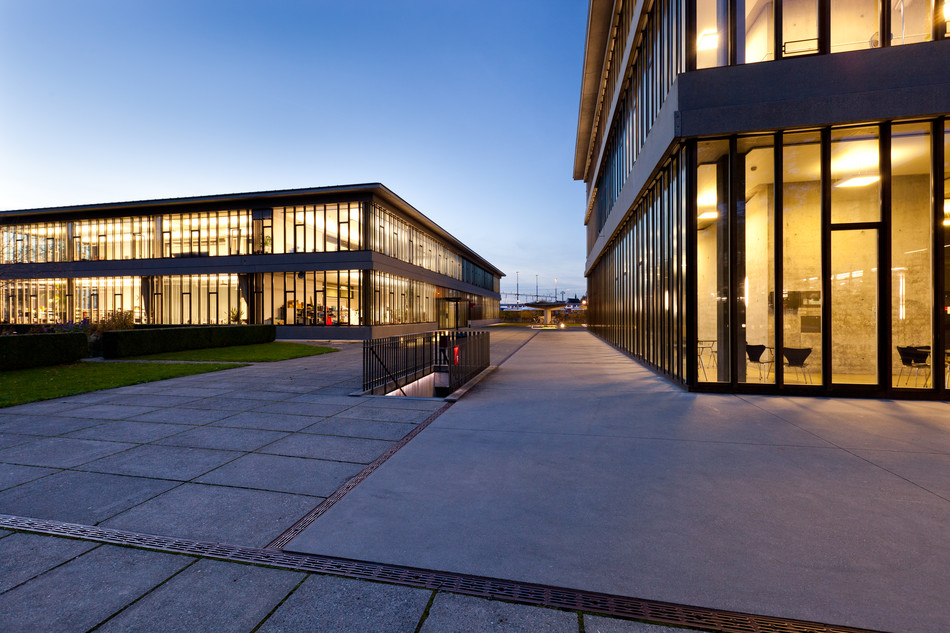
\includegraphics[height = 1cm]{images/hsr.jpg}}} %Kopfzeile links
	\fancyhead[C]{\textsl{\rightmark}} %zentrierte Kopfzeile
	\fancyhead[L]{\ifthenelse{\isodd{\value{page}}}{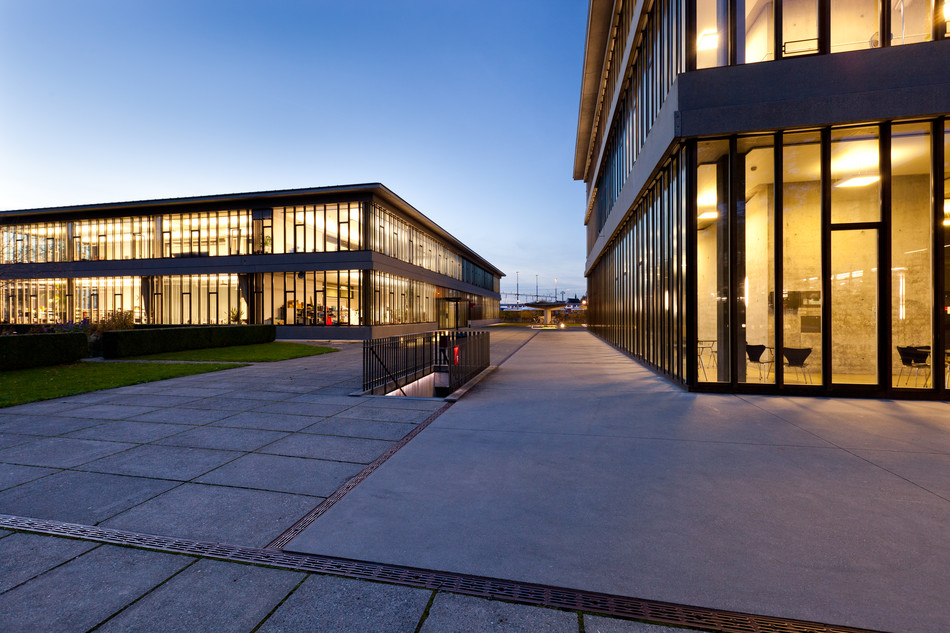
\includegraphics[height = 1cm]{images/hsr.jpg}}
								{
\includegraphics[height = 1cm]{header/hsrlogo.png}}} %Kopfzeile rechts
	\renewcommand{\headrulewidth}{0.4pt} %obere Trennlinie
	
	\fancyfoot[R]{\ifthenelse{\isodd{\value{page}}}{Seite \thepage\ / \pageref{LastPage}}{\today}}
	\fancyfoot[C]{\small{\Author}}
	\fancyfoot[L]{\ifthenelse{\isodd{\value{page}}}{\today}{Seite \thepage\ / \pageref{LastPage}}}
	\renewcommand{\footrulewidth}{0.4pt} %untere Trennlinie
}

\fancypagestyle{appendix}{
    \fancyhf{} %alle Kopf- und Fußzeilenfelder bereinigen
    \fancyhead[R]{} %Kopfzeile links
    \fancyhead[C]{} %zentrierte Kopfzeile
    \fancyhead[L]{} %Kopfzeile rechts
    \renewcommand{\headrulewidth}{0pt} %obere Trennlinie
    
    \fancyfoot[R]{\ifthenelse{\isodd{\value{page}}}{Seite \thepage\ / \pageref{LastPage}}{}}
    \fancyfoot[C]{}
    \fancyfoot[L]{\ifthenelse{\isodd{\value{page}}}{}{Seite \thepage\ / \pageref{LastPage}}}
    \renewcommand{\footrulewidth}{0.4pt} %untere Trennlinie
}

\pagestyle{plain} %Pagesytle


%%%%%%%%%%%%%%%%%%%%%
%% Load HSR Color  %%
%%%%%%%%%%%%%%%%%%%%%
\usepackage{xcolor}
\usepackage{header/HSRColors}

%%%%%%%%%%
% Colors %
%%%%%%%%%%
\definecolor{black}{rgb}{0,0,0}
\definecolor{red}{rgb}{1,0,0}
\definecolor{white}{rgb}{1,1,1}
\definecolor{grey}{rgb}{0.8,0.8,0.8}
\definecolor{green}{rgb}{0,.8,0.05}
\definecolor{brown}{rgb}{0.603,0,0}
\definecolor{mymauve}{rgb}{0.58,0,0.82}
\definecolor{mygreen}{RGB}{28,172,0}
\definecolor{mygray}{rgb}{0.5,0.5,0.5}
\definecolor{mymauve}{rgb}{0.58,0,0.82}
\definecolor{mylilas}{RGB}{170,55,241}

\definecolor{gray80}{gray}{0.8}
\definecolor{gray60}{gray}{0.6}
\definecolor{gray40}{gray}{0.4}
\definecolor{gray20}{gray}{0.2}

%%%%%%%%%%%%%%%%%%%%%
%% Title %%
%%%%%%%%%%%%%%%%%%%%%



%Title Spacing-----------------------------------------
\usepackage{titlesec}
%\titlespacing{name=\section}{-\marginparwidth}{0pt}{0.2em}
%\titlespacing{name=\subsection}{-\marginparwidth+10pt}{0pt}{0.2em}
%\titlespacing{name=\subsubsection}{-\marginparwidth+14pt}{0.2em}{0.2em}
%\titlespacing{name=\paragraph}{-\marginparwidth+18pt}{0.2em}{0.2em}

\titlespacing{name=\section}{1pt}{0pt}{0.2em}
\titlespacing{name=\subsection}{1pt}{0pt}{0.2em}
\titlespacing{name=\subsubsection}{1pt}{0.2em}{0.2em}
\titlespacing{name=\paragraph}{1pt}{0.2em}{0.2em}

%%%%%%%%%%%%%%%%%%
%% Bibliography %%
%%%%%%%%%%%%%%%%%%
%\usepackage[fixlanguage]{babelbib}
%\selectbiblanguage{german}
\usepackage[backend=bibtex,style=ieee, defernumbers=true]{biblatex} %Do not use biber with TexWorks
\addbibresource{Literatur}


% Abbildungen im Quellenverzeichnis nach Alphabet ordnen, Rest nummerieren
%\DeclareFieldFormat{labelnumber}{\ifkeyword{abb}{\mknumalph{#1}}{#1}}


%%%%%%%%%%%%%%%%%%%%%%%%%%%%%%%%%%%
%% Itemize and Enumerate spacing %%
%%%%%%%%%%%%%%%%%%%%%%%%%%%%%%%%%%%
% \topsep: space between first item and preceding paragraph
% \partopsep: extra space added to \topsep when environment starts a new paragraph
% \itemsep: space between successive items. 
\usepackage{enumitem} % Controls Layout of itemize, enumerate, description
\setlist[itemize]{topsep=0pt,itemsep=-1ex,partopsep=1ex,parsep=1ex,after=\vskip0.1\baselineskip}
\setlist[enumerate]{topsep=0pt,itemsep=-1ex,partopsep=1ex,parsep=1ex,after=\vskip0.1\baselineskip}

%%%%%%%%%%%
%% Index %%
%%%%%%%%%%%
\usepackage{imakeidx}
\makeindex[intoc,columnseprule]
\indexsetup{firstpagestyle=plain}    % Show header/footer on index page

%-------------------------------------------------
% Marginalien/Seitenränder
%-------------------------------------------------
%\marginpar{Eine Randnotiz}
\newcommand{\marg}[1]{\marginpar{\raggedright \textbf{#1} }}	

%%%%%%%%%%%%%%%%%%%%%%%
%% Aligned footnotes %%
%%%%%%%%%%%%%%%%%%%%%%%
\usepackage[hang]{footmisc}
\setlength{\footnotemargin}{1em}

%%%%%%%%%%%%%
%% Tabular %%
%%%%%%%%%%%%%
\newcolumntype{L}[1]{>{\raggedright\arraybackslash}p{#1}} % Tabelleninhalt linksausgerichtet
\newcolumntype{R}[1]{>{\raggedleft\arraybackslash}p{#1}} % Tabelleninhalt rechtsausgerichtet
\newcolumntype{C}[1]{>{\centering\arraybackslash}p{#1}} %  Tabelleninhalt zentriert


%%%%%%%%%%%%%%%%%%%%%%
%% Generelle Makros %%
%%%%%%%%%%%%%%%%%%%%%%

% If \Print=true, then make all links black for nicer print
\providecommand*{\True}{true}
\ifx \Print \True
\hypersetup{hidelinks, colorlinks, linkcolor = black, citecolor = black, filecolor = black, urlcolor = black}
\fi

\parindent0pt % Zeileneinzug verhindern

%Matlab font
\newcommand{\matlab}[1]{\footnotesize{(Matlab: \texttt{#1})}\normalsize{}}

% Makro für Tabellenbilder gleich unterhalb der Linie
\newcommand\tabbild[2][]{%
	\raisebox{0pt}[\dimexpr\totalheight+\dp\strutbox\relax][\dp\strutbox]{%
		\includegraphics[#1]{#2}%
	}%
}

% Makro für Vorteile und Nachteil mit Plus und Minus
\newcommand\pro{\item[$+$]}
\newcommand\con{\item[$-$]}


%Float-Barrier for Subsection
\makeatletter
\AtBeginDocument{%
	\expandafter\renewcommand\expandafter\subsection\expandafter{%
		\expandafter\@fb@secFB\subsection
	}%
}
\makeatother


%%%%%%%%%%%%%%%%%%%%%%%%%%%%
% Mathematical Operators %
%%%%%%%%%%%%%%%%%%%%%%%%%%%%
\DeclareMathOperator{\sinc}{sinc}
\DeclareMathOperator{\sgn}{sgn}
\DeclareMathOperator{\Real}{Re}
\DeclareMathOperator{\Imag}{Im}
\DeclareMathOperator{\euler}{e}
\DeclareMathOperator{\cov}{cov}
\DeclareMathOperator{\PolyGrad}{PolyGrad}
\DeclareMathOperator{\gradient}{grad}
\DeclareMathOperator{\rotation}{rot}
\DeclareMathOperator{\divergenz}{div}
\DeclareMathOperator{\imag}{j}

%Grösse Integral anpassen
\def\Int{\mbox{\Large$\displaystyle\int$\normalsize}}
\def\Int{\mbox{\Large$\displaystyle\iint$\normalsize}}
\def\OInt{\mbox{\Large$\displaystyle\oint$\normalsize}}

%Makro für 'd' von Integral- und Differentialgleichungen 
\newcommand*{\diff}{\mathop{}\!\mathrm{d}}

%%%%%%%%%%%%%%%%%%%%%%%%%%%
% Fouriertransform %
%%%%%%%%%%%%%%%%%%%%%%%%%%%

\unitlength1cm
\newcommand{\FT}
{
	\begin{picture}(1,0.5)
	\put(0.2,0.1){\circle{0.14}}\put(0.27,0.1){\line(1,0){0.5}}\put(0.77,0.1){\circle*{0.14}}
	\end{picture}
}


\newcommand{\IFT}
{
	\begin{picture}(1,0.5)
	\put(0.2,0.1){\circle*{0.14}}\put(0.27,0.1){\line(1,0){0.45}}\put(0.77,0.1){\circle{0.14}}
	\end{picture}
}


